\documentclass[hide notes,intlimits,usenames,dvipsnames]{beamer}

\mode<presentation>
{
  \usetheme{Singapore}
  \usefonttheme{professionalfonts}
  \setbeamertemplate{blocks}[rounded][shadow=true]
  \setbeamercovered{transparent}
  \setbeamertemplate{footline}[frame number]
}

% load packages
\usepackage[english]{babel}
\usepackage[latin1]{inputenc}
\usepackage[T1]{fontenc}
\usepackage{lmodern}
\usepackage[multidot]{grffile}
\usepackage{verbatim,empheq}

\usepackage{tikz}
\usetikzlibrary{shapes,arrows,shadows}
\usetikzlibrary{decorations.pathreplacing}

\usepackage{animate}
\usepackage{amsmath,verbatim}

% see http://tex.stackexchange.com/questions/86188/labelling-with-arrows-in-an-automated-way

\newif\ifclipme\clipmetrue
\tikzset{labelstyle/.style={LabelStyle/.append style={#1}},linestyle/.style={LineStyle/.append style={#1}}}
\tikzset{LabelStyle/.initial={},LineStyle/.initial={}}

\newcommand{\mathWithDescription}[4][]{{%
    \tikzset{#1}%
    \tikz[baseline]{
        \node[draw=red,rounded corners,anchor=base] (m#4) {$\displaystyle#2$};
        \ifclipme\begin{pgfinterruptboundingbox}\fi
            \node[above of=m#4,font=\strut, LabelStyle] (l#4) {#3};
            \draw[-,red, LineStyle] (l#4) to (m#4);
        \ifclipme\end{pgfinterruptboundingbox}\fi
    }%
}}

\newcommand{\mathWithDescriptionStarred}[3][]{{%
    \clipmefalse%
    \mathWithDescription[#1]{#2}{#3}{\themathLabelNode}%
}}

\newcounter{mathLabelNode}

\newcommand{\mathLabelBox}[3][]{%
   \stepcounter{mathLabelNode}%
   \mathWithDescription[#1]{#2}{#3}{\themathLabelNode}%
   \vphantom{\mathWithDescriptionStarred[#1]{#2}{#3}{\themathLabelNode}}%
}

\definecolor{dark red}{HTML}{E41A1C}
\definecolor{dark green}{HTML}{4DAF4A}
\definecolor{dark violet}{HTML}{984EA3}
\definecolor{dark blue}{HTML}{084594}
\definecolor{dark orange}{HTML}{FF7F00}
\definecolor{light blue}{HTML}{377EB8}
\definecolor{light red}{HTML}{FB9A99}
\definecolor{light violet}{HTML}{CAB2D6}

\newcommand{\CC}{\mathbb{C}}
\newcommand{\NN}{\mathbb{N}}
\newcommand{\RR}{\mathbb{R}}
\newcommand{\ZZ}{\mathbb{Z}}

\newcommand{\Kcal}{\mathcal{K}}
\newcommand{\Xcal}{\mathcal{X}}

\newcommand{\bF}{\mathbf{F}}
\newcommand{\bQ}{\mathbf{Q}}
\newcommand{\bU}{\mathbf{U}}
\newcommand{\bX}{\mathbf{X}}

\newcommand{\bn}{\mathbf{n}}
\newcommand{\bq}{\mathbf{q}}
\newcommand{\bu}{\mathbf{u}}
\newcommand{\bv}{\mathbf{v}}
\newcommand{\bx}{\mathbf{x}}

\newcommand{\Div}{\nabla\cdot}
\newcommand{\eps}{\epsilon}
\newcommand{\grad}{\nabla}
\newcommand{\lap}{\triangle}
\renewcommand{\bar}{\overline}

\newcommand{\ip}[2]{\ensuremath{\left<#1,#2\right>}}

\newcommand{\Span}{\operatorname{span}}

\newenvironment{transbox}[1][]{%
\begin{tikzpicture}
\node[drop shadow,rounded corners,text width=\textwidth,fill=white, fill opacity=#1,text opacity=1] \bgroup
}{
\egroup;\end{tikzpicture}}


\title{A practical view of the FEM}

\subtitle{with some software}

\author[Bueler]{Ed Bueler}

\institute[UAF]{
  \scriptsize Dept of Mathematics and Statistics \\

  University of Alaska Fairbanks
}

%\titlegraphic{\includegraphics[width=\textwidth]{andycoast.png}}

\beamertemplatenavigationsymbolsempty   % remove faint and silly navigation symbols at bottom
\renewcommand{\insertnavigation}[1]{}   % remove section headings from top of each slide

\setbeamerfont{date}{size=\scriptsize}
\date{}

%\AtBeginSection[]
%{
%  \begin{frame}<beamer>
%    \frametitle{Outline}
%    %\tableofcontents[currentsection,hideallsubsections]
%    \tableofcontents[currentsection]
%  \end{frame}
%}


\begin{document}

\begin{frame}
\vspace{10mm}
  \titlepage
  \begin{center}
  \tiny DMS \hfill 27 November 2018
  \end{center}
\end{frame}


\begin{frame}
    \frametitle{Outline}
    \tableofcontents
\end{frame}

\section{assembly}

\begin{frame}{general Poisson problem}
\begin{itemize}
\item $\Omega \subset \RR^2$ % with disjoint decomposition $\partial \Omega = \partial_D \Omega \cup \partial_N \Omega$
\item generalize our usual ``$\triangle u = f$, $u=0$ on $\partial\Omega$'' problem:
\begin{align*}
- \Div \left(a(u) \grad u\right) &= f(u)  &&\text{ on } \Omega, \\
u &= g_D &&\text{ on } \partial_D \Omega, \notag \\
\frac{\partial u}{\partial n} &= g_N &&\text{ on } \partial_N \Omega. \notag
\end{align*}
\item $a(u,x,y)$, $f(u,x,y)$, $g_N(x,y)$, $g_D(x,y)$ are given (data)
%\item for well-posedness:
%    \begin{itemize}
%    \item[$\circ$] assume $a,f,g_N,g_D$ at least $L^2$ in $x,y$
%    \item[$\circ$] expect $f$ to be Lipschitz in $u$
%    \item[$\circ$] assume \emph{uniform ellipticity}: $a(u,x,y) \ge \eps > 0$
%    \end{itemize}
\end{itemize}
\end{frame}

\begin{frame}{general Poisson problem}
\begin{center}
\input{generalpoissondomain.tex}
\end{center}
\end{frame}

\begin{frame}{weak form}
\begin{itemize}
\item $u\in H_g^1(\Omega) = \{u\in H^1(\Omega)\,:\,u=g_D \text{ on } \partial_D\Omega\}$
\item test functions: $H_0^1(\Omega) = \{v\in H^1(\Omega)\,:\,v=0 \text{ on } \partial_D\Omega\}$
\item for $v\in H^1_0(\Omega)$, multiply PDE by $v$ and integrate by parts:
\begin{equation*}
\int_\Omega a(u) \grad u \cdot \grad v - \int_{\partial\Omega} \frac{\partial u}{\partial n} v = \int_\Omega f(u) v
\end{equation*}
\item apply boundary conditions:
\begin{equation*}
\int_\Omega a(u) \grad u \cdot \grad v = \int_\Omega f(u) v + \int_{\partial_N\Omega} g_N v \tag{WF}
\end{equation*}
\item seek $u \in H^1_g(\Omega)$ satisfying weak form (WF)
\item Neumann data $g_N$ appears in (WF)
\item Dirichlet data $g_D$ is used in defining $H^1_g(\Omega)$
\end{itemize}
\end{frame}

\begin{frame}{examples of such PDEs}
\begin{itemize}
\item Poisson equation:
    $$-\triangle u=f(x,y), \quad u=0 \text{ on } \partial \Omega$$
\item Liouville-Bratu equation:
    $$-\triangle u = \lambda e^u$$

\vspace{-3mm}
    \begin{itemize}
    \item[$\circ$] critical $\lambda$ for well-posedness
    \end{itemize}
\item porous-medium equation:
    $$-\Div\left((u^{m-1} + \eps)\grad u\right) = f$$

\vspace{-3mm}
    \begin{itemize}
    \item[$\circ$] regularized with $\eps>0$ for uniform ellipticity
    \end{itemize}
\end{itemize}
\end{frame}

\begin{frame}{triangulation and numbering}
\mbox{% created by command line:
%   tmp/petsc2tikz.py --labelelements --nodesize 1.0 --dirichletsize 3.0 --scale 0.63 tmp/blob1 -o tmp/blob1_elenum.tikz
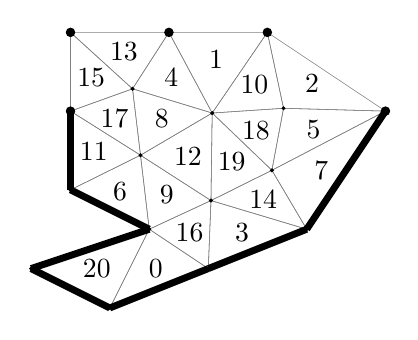
\begin{tikzpicture}[scale=0.5]
  \draw[gray,very thin] (2.000000,-3.000000) -- (3.500000,-4.000000) -- (1.000000,-5.000000) -- (2.000000,-3.000000) ;
  \draw (2.166667,-4.000000) node {$0$};
  \draw[gray,very thin] (5.000000,2.000000) -- (3.598633,-0.048909) -- (2.500000,2.000000) -- (5.000000,2.000000) ;
  \draw (3.699544,1.317030) node {$1$};
  \draw[gray,very thin] (5.000000,2.000000) -- (8.000000,0.000000) -- (5.410836,0.072145) -- (5.000000,2.000000) ;
  \draw (6.136945,0.690715) node {$2$};
  \draw[gray,very thin] (6.000000,-3.000000) -- (3.500000,-4.000000) -- (3.567839,-2.271643) -- (6.000000,-3.000000) ;
  \draw (4.355946,-3.090548) node {$3$};
  \draw[gray,very thin] (2.500000,2.000000) -- (3.598633,-0.048909) -- (1.575312,0.566253) -- (2.500000,2.000000) ;
  \draw (2.557982,0.839115) node {$4$};
  \draw[gray,very thin] (5.410836,0.072145) -- (8.000000,0.000000) -- (5.115191,-1.502985) -- (5.410836,0.072145) ;
  \draw (6.175342,-0.476947) node {$5$};
  \draw[gray,very thin] (2.000000,-3.000000) -- (0.000000,-2.000000) -- (1.777927,-1.119826) -- (2.000000,-3.000000) ;
  \draw (1.259309,-2.039942) node {$6$};
  \draw[gray,very thin] (8.000000,0.000000) -- (6.000000,-3.000000) -- (5.115191,-1.502985) -- (8.000000,0.000000) ;
  \draw (6.371730,-1.500995) node {$7$};
  \draw[gray,very thin] (3.598633,-0.048909) -- (1.777927,-1.119826) -- (1.575312,0.566253) -- (3.598633,-0.048909) ;
  \draw (2.317291,-0.200827) node {$8$};
  \draw[gray,very thin] (2.000000,-3.000000) -- (1.777927,-1.119826) -- (3.567839,-2.271643) -- (2.000000,-3.000000) ;
  \draw (2.448589,-2.130490) node {$9$};
  \draw[gray,very thin] (5.000000,2.000000) -- (5.410836,0.072145) -- (3.598633,-0.048909) -- (5.000000,2.000000) ;
  \draw (4.669823,0.674412) node {$10$};
  \draw[gray,very thin] (0.000000,0.000000) -- (1.777927,-1.119826) -- (0.000000,-2.000000) -- (0.000000,0.000000) ;
  \draw (0.592642,-1.039942) node {$11$};
  \draw[gray,very thin] (3.598633,-0.048909) -- (3.567839,-2.271643) -- (1.777927,-1.119826) -- (3.598633,-0.048909) ;
  \draw (2.981466,-1.146793) node {$12$};
  \draw[gray,very thin] (0.000000,2.000000) -- (2.500000,2.000000) -- (1.575312,0.566253) -- (0.000000,2.000000) ;
  \draw (1.358437,1.522084) node {$13$};
  \draw[gray,very thin] (6.000000,-3.000000) -- (3.567839,-2.271643) -- (5.115191,-1.502985) -- (6.000000,-3.000000) ;
  \draw (4.894343,-2.258209) node {$14$};
  \draw[gray,very thin] (0.000000,0.000000) -- (0.000000,2.000000) -- (1.575312,0.566253) -- (0.000000,0.000000) ;
  \draw (0.525104,0.855418) node {$15$};
  \draw[gray,very thin] (2.000000,-3.000000) -- (3.567839,-2.271643) -- (3.500000,-4.000000) -- (2.000000,-3.000000) ;
  \draw (3.022613,-3.090548) node {$16$};
  \draw[gray,very thin] (0.000000,0.000000) -- (1.575312,0.566253) -- (1.777927,-1.119826) -- (0.000000,0.000000) ;
  \draw (1.117746,-0.184524) node {$17$};
  \draw[gray,very thin] (3.598633,-0.048909) -- (5.410836,0.072145) -- (5.115191,-1.502985) -- (3.598633,-0.048909) ;
  \draw (4.708220,-0.493250) node {$18$};
  \draw[gray,very thin] (3.598633,-0.048909) -- (5.115191,-1.502985) -- (3.567839,-2.271643) -- (3.598633,-0.048909) ;
  \draw (4.093888,-1.274512) node {$19$};
  \draw[gray,very thin] (2.000000,-3.000000) -- (1.000000,-5.000000) -- (-1.000000,-4.000000) -- (2.000000,-3.000000) ;
  \draw (0.666667,-4.000000) node {$20$};
  \filldraw (0.000000,0.000000) circle (3.000000pt);
  \filldraw (0.000000,2.000000) circle (3.000000pt);
  \filldraw (5.000000,2.000000) circle (3.000000pt);
  \filldraw (8.000000,0.000000) circle (3.000000pt);
  \filldraw (6.000000,-3.000000) circle (1.000000pt);
  \filldraw (1.000000,-5.000000) circle (1.000000pt);
  \filldraw (-1.000000,-4.000000) circle (1.000000pt);
  \filldraw (2.000000,-3.000000) circle (1.000000pt);
  \filldraw (0.000000,-2.000000) circle (1.000000pt);
  \filldraw (2.500000,2.000000) circle (3.000000pt);
  \filldraw (3.500000,-4.000000) circle (1.000000pt);
  \filldraw (3.598633,-0.048909) circle (1.000000pt);
  \filldraw (1.777927,-1.119826) circle (1.000000pt);
  \filldraw (3.567839,-2.271643) circle (1.000000pt);
  \filldraw (5.410836,0.072145) circle (1.000000pt);
  \filldraw (1.575312,0.566253) circle (1.000000pt);
  \filldraw (5.115191,-1.502985) circle (1.000000pt);
  \draw[line width=2.500000pt] (8.000000,0.000000) -- (6.000000,-3.000000);
  \draw[line width=2.500000pt] (6.000000,-3.000000) -- (3.500000,-4.000000);
  \draw[line width=2.500000pt] (3.500000,-4.000000) -- (1.000000,-5.000000);
  \draw[line width=2.500000pt] (1.000000,-5.000000) -- (-1.000000,-4.000000);
  \draw[line width=2.500000pt] (-1.000000,-4.000000) -- (2.000000,-3.000000);
  \draw[line width=2.500000pt] (2.000000,-3.000000) -- (0.000000,-2.000000);
  \draw[line width=2.500000pt] (0.000000,-2.000000) -- (0.000000,0.000000);
\end{tikzpicture}
 \quad % created by command line:
%   tmp/petsc2tikz.py --labelnodes --nodesize 1.0 --dirichletsize 3.0 --nodeoffset -0.5 --scale 0.63 tmp/blob1 -o tmp/blob1_nodenum.tikz
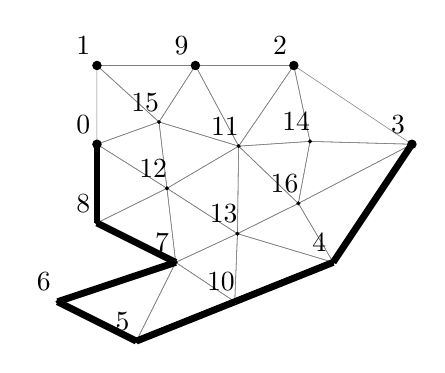
\begin{tikzpicture}[scale=0.5]
  \draw[gray,very thin] (2.000000,-3.000000) -- (3.500000,-4.000000) -- (1.000000,-5.000000) -- (2.000000,-3.000000) ;
  \draw[gray,very thin] (5.000000,2.000000) -- (3.598633,-0.048909) -- (2.500000,2.000000) -- (5.000000,2.000000) ;
  \draw[gray,very thin] (5.000000,2.000000) -- (8.000000,0.000000) -- (5.410836,0.072145) -- (5.000000,2.000000) ;
  \draw[gray,very thin] (6.000000,-3.000000) -- (3.500000,-4.000000) -- (3.567839,-2.271643) -- (6.000000,-3.000000) ;
  \draw[gray,very thin] (2.500000,2.000000) -- (3.598633,-0.048909) -- (1.575312,0.566253) -- (2.500000,2.000000) ;
  \draw[gray,very thin] (5.410836,0.072145) -- (8.000000,0.000000) -- (5.115191,-1.502985) -- (5.410836,0.072145) ;
  \draw[gray,very thin] (2.000000,-3.000000) -- (0.000000,-2.000000) -- (1.777927,-1.119826) -- (2.000000,-3.000000) ;
  \draw[gray,very thin] (8.000000,0.000000) -- (6.000000,-3.000000) -- (5.115191,-1.502985) -- (8.000000,0.000000) ;
  \draw[gray,very thin] (3.598633,-0.048909) -- (1.777927,-1.119826) -- (1.575312,0.566253) -- (3.598633,-0.048909) ;
  \draw[gray,very thin] (2.000000,-3.000000) -- (1.777927,-1.119826) -- (3.567839,-2.271643) -- (2.000000,-3.000000) ;
  \draw[gray,very thin] (5.000000,2.000000) -- (5.410836,0.072145) -- (3.598633,-0.048909) -- (5.000000,2.000000) ;
  \draw[gray,very thin] (0.000000,0.000000) -- (1.777927,-1.119826) -- (0.000000,-2.000000) -- (0.000000,0.000000) ;
  \draw[gray,very thin] (3.598633,-0.048909) -- (3.567839,-2.271643) -- (1.777927,-1.119826) -- (3.598633,-0.048909) ;
  \draw[gray,very thin] (0.000000,2.000000) -- (2.500000,2.000000) -- (1.575312,0.566253) -- (0.000000,2.000000) ;
  \draw[gray,very thin] (6.000000,-3.000000) -- (3.567839,-2.271643) -- (5.115191,-1.502985) -- (6.000000,-3.000000) ;
  \draw[gray,very thin] (0.000000,0.000000) -- (0.000000,2.000000) -- (1.575312,0.566253) -- (0.000000,0.000000) ;
  \draw[gray,very thin] (2.000000,-3.000000) -- (3.567839,-2.271643) -- (3.500000,-4.000000) -- (2.000000,-3.000000) ;
  \draw[gray,very thin] (0.000000,0.000000) -- (1.575312,0.566253) -- (1.777927,-1.119826) -- (0.000000,0.000000) ;
  \draw[gray,very thin] (3.598633,-0.048909) -- (5.410836,0.072145) -- (5.115191,-1.502985) -- (3.598633,-0.048909) ;
  \draw[gray,very thin] (3.598633,-0.048909) -- (5.115191,-1.502985) -- (3.567839,-2.271643) -- (3.598633,-0.048909) ;
  \draw[gray,very thin] (2.000000,-3.000000) -- (1.000000,-5.000000) -- (-1.000000,-4.000000) -- (2.000000,-3.000000) ;
  \filldraw (0.000000,0.000000) circle (3.000000pt);
  \draw (-0.350000,0.500000) node {$0$};
  \filldraw (0.000000,2.000000) circle (3.000000pt);
  \draw (-0.350000,2.500000) node {$1$};
  \filldraw (5.000000,2.000000) circle (3.000000pt);
  \draw (4.650000,2.500000) node {$2$};
  \filldraw (8.000000,0.000000) circle (3.000000pt);
  \draw (7.650000,0.500000) node {$3$};
  \filldraw (6.000000,-3.000000) circle (1.000000pt);
  \draw (5.650000,-2.500000) node {$4$};
  \filldraw (1.000000,-5.000000) circle (1.000000pt);
  \draw (0.650000,-4.500000) node {$5$};
  \filldraw (-1.000000,-4.000000) circle (1.000000pt);
  \draw (-1.350000,-3.500000) node {$6$};
  \filldraw (2.000000,-3.000000) circle (1.000000pt);
  \draw (1.650000,-2.500000) node {$7$};
  \filldraw (0.000000,-2.000000) circle (1.000000pt);
  \draw (-0.350000,-1.500000) node {$8$};
  \filldraw (2.500000,2.000000) circle (3.000000pt);
  \draw (2.150000,2.500000) node {$9$};
  \filldraw (3.500000,-4.000000) circle (1.000000pt);
  \draw (3.150000,-3.500000) node {$10$};
  \filldraw (3.598633,-0.048909) circle (1.000000pt);
  \draw (3.248633,0.451091) node {$11$};
  \filldraw (1.777927,-1.119826) circle (1.000000pt);
  \draw (1.427927,-0.619826) node {$12$};
  \filldraw (3.567839,-2.271643) circle (1.000000pt);
  \draw (3.217839,-1.771643) node {$13$};
  \filldraw (5.410836,0.072145) circle (1.000000pt);
  \draw (5.060836,0.572145) node {$14$};
  \filldraw (1.575312,0.566253) circle (1.000000pt);
  \draw (1.225312,1.066253) node {$15$};
  \filldraw (5.115191,-1.502985) circle (1.000000pt);
  \draw (4.765191,-1.002985) node {$16$};
  \draw[line width=2.500000pt] (8.000000,0.000000) -- (6.000000,-3.000000);
  \draw[line width=2.500000pt] (6.000000,-3.000000) -- (3.500000,-4.000000);
  \draw[line width=2.500000pt] (3.500000,-4.000000) -- (1.000000,-5.000000);
  \draw[line width=2.500000pt] (1.000000,-5.000000) -- (-1.000000,-4.000000);
  \draw[line width=2.500000pt] (-1.000000,-4.000000) -- (2.000000,-3.000000);
  \draw[line width=2.500000pt] (2.000000,-3.000000) -- (0.000000,-2.000000);
  \draw[line width=2.500000pt] (0.000000,-2.000000) -- (0.000000,0.000000);
\end{tikzpicture}
}

\begin{itemize}
\item triangulation $\mathcal{T}_h$ of a polygon $\Omega$
\item numbering:
    \begin{itemize}
    \item[$\circ$] $K=21$ elements (left)
    \item[$\circ$] $N=17$ nodes (right)
    \item[$\circ$] $P=7$ segments in Neumann boundary (bold)
    \item[$\circ$] $n_D=5$ nodes in Dirichlet boundary
    \end{itemize}
\end{itemize}
\end{frame}

\begin{frame}{FEM spaces}
\vspace{4mm}

\begin{itemize}
\item hat functions satisfy $\psi_j(\bx_i)=\delta_{ij}$

\vspace{-10mm}

\hfill     % (2,2,1) is top
    \draw (0,0,0) -- (2,2,1); % to top from left
    \draw (4,0,0) -- (2,2,1); %   ...  from front
    \draw (4,0,3) -- (2,2,1); %   ...  from right
    \draw[color=gray] (0.3,0,4) -- (2,2,1); % from back
    \draw[color=gray] (2,0.4,1) -- (2,2,1); % from middle

    % draw base
    \draw (0,0,0) -- (4,0,0);
    \draw (4,0,0) -- (4,0,3);
    \draw[color=gray] (0,0,0) -- (0.3,0,4);
    \draw[color=gray] (0.3,0,4) -- (4,0,3);
    \draw[color=gray] (0,0,0) -- (2,0.4,1);
    \draw[color=gray] (2,0.4,1) -- (4,0,3);
    \draw[color=gray] (4,0,0) -- (2,0.4,1);
    \draw[color=gray] (2,0.4,1) -- (0.3,0,4);

    % extend flat
    \draw (0,0,0) -- (-0.7,-0.7,0);
    \draw (0,0,0) -- (1.5,-0.6,0);
    \draw (0,0,0) -- (-1,0.6,0);
    \draw (4,0,0) -- (1.5,-0.6,0);
    \draw (4,0,0) -- (5.5,0.1,0);
    \draw (4,0,0) -- (5,-0.5,0);
    \draw (4,0,3) -- (5.5,0.1,0);
    \draw (4,0,3) -- (5,0,2);

    % label node j
    \draw (2,2,1.9) node {{\scriptsize $\psi_j=1$}};
    \draw (2,0.15,0.8) node {{\scriptsize node $j$}};
    \draw (2,0.4,1) circle (4.0pt);

    % draw nodes
    \filldraw[color=gray] (0.3,0,4) circle (0.8pt);
    \filldraw[color=gray] (2,0.4,1) circle (1.0pt);
    \filldraw (4,0,3) circle (1.0pt);
    \filldraw (0,0,0) circle (1.25pt);
    \filldraw (4,0,0) circle (1.25pt);
    \filldraw (5.5,0.1,0) circle (1.25pt);
    \filldraw (1.5,-0.6,0) circle (1.5pt);

\item use hat functions to approximate $g_D(\bx)$:
\begin{equation*}
\hat g_D(x,y) = \sum_{l=0}^{n_D-1} g_D(\bx_{j_l}) \psi_{j_l}(x,y) \quad \in C(\overline\Omega)
\end{equation*}
\item use hat functions to define test functions:
\begin{equation*}
S_{0}^h = \Span\left<\psi_j \,:\, \bx_j \notin \partial_D \Omega\right> \subset H_0^1(\Omega)
\end{equation*}
\item and trial functions
\begin{equation*}
S_{g}^h = \left\{\hat g_D + w \,:\, w \in S_{0}^h\right\} \subset H_g^1(\Omega)
\end{equation*}
\end{itemize}
\end{frame}

\begin{frame}{FEM spaces}
\begin{itemize}
\item expand the trial function $u^h$:
\begin{equation*}
u^h(x,y) = \hat g_D(x,y) + \sum_{\bx_j \notin \partial_D \Omega} u_j\, \psi_j(x,y)
\end{equation*}
\item for all $i$ such that $\bx_i \notin \partial_D \Omega$,
\begin{equation*}
\int_\Omega a(u^h) \grad u^h \cdot \grad \psi_i = \int_\Omega f(u^h) \psi_i + \int_{\partial_N\Omega} g_N \psi_i
\end{equation*}
\item $\dim(S_{0}^h)=\dim(S_{g}^h)=N-n_D$
\end{itemize}
\end{frame}

\section{solving the equations}

\begin{frame}{X}
X
\end{frame}

\begin{frame}{X}
X
\end{frame}

\section{runtime choices}

\begin{frame}{X}
X
\end{frame}

\begin{frame}{X}
X
\end{frame}

\begin{frame}{X}
X
\end{frame}

\begin{frame}{X}
X
\end{frame}

\begin{frame}{X}
X
\end{frame}

\begin{frame}{X}
X
\end{frame}


\end{document}
